\newcommand{\doctitle}{Construct and Destroy \\ Software Architecture}
\newcommand{\doctitleshort}{C\&D Software Architecture}

\newcommand{\docauthor} {
    \renewcommand{\arraystretch}{0.5}
    \begin{tabular}{l l}
        \textbf{Students:} & ~ \\
        Mark van der Woude     & {\mdseries(S1081655)} \\
        Stephan Schrijver     & {\mdseries(S1078783)} \\
        Jeroen Vinke     & {\mdseries(S1078666)} \\
        Sander Bouwman   & {\mdseries(S1080528)} \\
        Robin T. Koning  & {\mdseries(S1078710)} \\
    \end{tabular}
}

\newcommand{\doctitlepage} {
    \thispagestyle{empty}
    \parbox[t]{1.0\linewidth}{
        \fontsize{40pt}{60pt}\selectfont
        \vspace*{1.5cm}
        \doctitle{}
        \vspace*{1.5cm}
    }
    \vfill
    {
        \centering
        \large
        \hfill \today
        \hfill \docauthor{}
    }
    \normalcolor{}

    \newpage
}

\providecommand{\doctitle}{Title}
\providecommand{\docauthor}{Author}
\providecommand{\doctype}{scrartcl}
\providecommand{\doctitlepage}{TitlePage}

\documentclass[12pt,a4paper,titlepage,parskip=full]{\doctype}

\usepackage[english]{babel}
\usepackage{caption}
\usepackage{float}
\usepackage{blindtext}
\usepackage{hyperref}
\usepackage{graphicx}
\usepackage{listings}
\usepackage{tikz}
\usetikzlibrary{decorations.pathreplacing}
\usepackage{pdfpages}
\usepackage{apacite}
\usepackage{listings}
\bibliographystyle{apacite}

% Input and output encoding ---------------------------------------------------
\usepackage{iftex}
\ifPDFTeX
   \usepackage[utf8]{inputenc}
   \usepackage[T1]{fontenc}
   \usepackage{lmodern}
\else
   \ifXeTeX
     \usepackage{xltxtra}
   \else
     \usepackage{luatextra}
   \fi
   \defaultfontfeatures{Ligatures=TeX}
\fi

% Math
\usepackage{amsmath}
\usepackage{amsfonts}
\usepackage{amsthm}
\usepackage{amssymb}
\usepackage{mathtools}
\usepackage{bm}
\newcommand{\uvec}[1]{\boldsymbol{\hat{\textbf{#1}}}}

\DeclarePairedDelimiter{\ceil}{\lceil}{\rceil}
\DeclarePairedDelimiter{\floor}{\lfloor}{\rfloor}
\DeclarePairedDelimiter{\bag}{\langle}{\rangle}
\DeclarePairedDelimiter{\set}{\{}{\}}

% Misc
\usepackage{marginnote}
\usepackage[shortlabels]{enumitem}

% Display
\usepackage{lastpage}
\usepackage{fancyhdr}
\setlength{\headheight}{24pt}
\usepackage{eurosym}
\pagestyle{fancy}

\usepackage[nameinlink]{cleveref}

\title{\doctitle}
\author{\docauthor}
\date{\today}

\lhead{\doctitleshort}
\rhead{\today}
\cfoot{\thepage\ /~\pageref{LastPage}}
%\lfoot{\docauthor}

\numberwithin{equation}{section}
\numberwithin{figure}{section}
\numberwithin{table}{section}

\usepackage{changepage}

%Other settings
\lstset{basicstyle=\ttfamily}

\begin{document}
\doctitlepage{}

\tableofcontents
\thispagestyle{empty}
\newpage

\clearpage
\setcounter{page}{1}
\addtocontents{toc}{\protect\thispagestyle{empty}}
\newpage

% Abstract, the intro to our document
\begin{abstract}
\blindtext
\end{abstract}

\newpage

%----------------------------------
% Put new chapters in this block


\section{Controlling workers}

One of the things the player can do is order workers to do a specific task. This is done by selecting one or more workers followed by right clicking somewhere. For example, the player can right click on the ground, which will cause the selected workers to move there. The player can also order workers to gather resources such as wood.

Since the player can select any kind of worker and order it to do many different things, a design pattern was needed to ensure that the code remained readable and extensible. The strategy pattern was chosen because of the fact that it is very extensible. 

A class diagram of relevant classes can be found in \cref{fig:orderstrategies}. The basic idea is that there is one singleton class named MoveOrder with a orderMove function. This function can be used throughout the game to order one or more entities to do something at a certain vector. Based on what the player right clicked on an OrderStrategy is selected. This OrderStrategy takes care of the right click event, for example by ordering the selected entities to go to a certain location.

Down below, in \cref{fig:orderstrategy}, you can find the implementation of the strategy that handles the event where a user orders one or more entities to move to a piece of ground.

\begin{figure}[!htb]
    \centering
    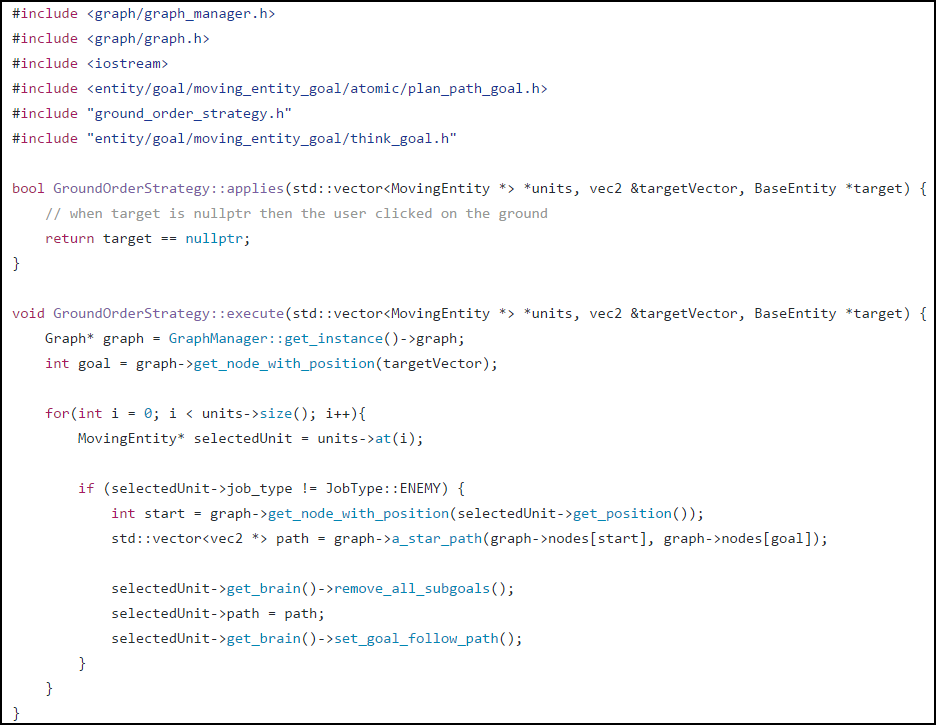
\includegraphics[angle=0,origin=c,scale=0.66]
    {images/order-strategy.PNG}
    \caption{Order strategy}\label{fig:orderstrategy}
\end{figure}


\newpage

%----------------------------------

\bibliography{bib/sources}
\newpage

\section{Appendix}
\begin{figure}[!htb]
    \centering
    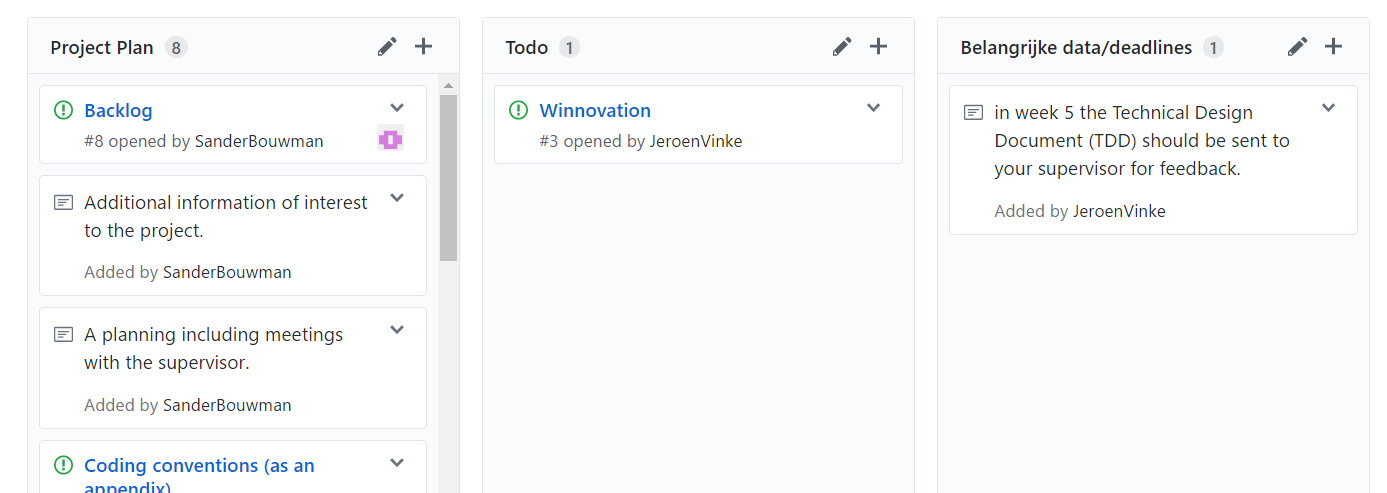
\includegraphics[angle=-90,origin=c,scale=0.75]
    {images/github-projects.PNG}
    \caption{GitHub project}\label{fig:githubproject}
\end{figure}

\end{document}

